\documentclass{article}

\usepackage{amsmath}
\usepackage{graphicx}
\usepackage{subcaption}
\usepackage{listings}
\usepackage{xcolor}
\usepackage{algorithm}
\usepackage{algorithmicx}
\usepackage{algpseudocode}
\usepackage{array}
\usepackage{tikz}
\usetikzlibrary{3d}
\usepackage{float}
\usepackage{natbib}
\usepackage{booktabs}

\usepackage{graphicx}
\graphicspath{ {./pics/} }

\lstdefinestyle{mystyle}{
    language=Python,
    basicstyle=\ttfamily,
    keywordstyle=\color{blue},
    commentstyle=\color{green},
    numbers=left,
    numberstyle=\tiny,
    stepnumber=1,
    tabsize=2,
    frame=single,
    breaklines=true,
    captionpos=b,
    showstringspaces=false,
}

\title{Leveraging Surface Normal Distributions for Fast 3D Object Recognition: A Point Cloud-Based Approach}

\author{
  Eduardo Di Santi
}

\date{\today}

\begin{document}
\maketitle

\begin{abstract}
    This paper presents a novel and efficient method for 3D object recognition and similarity determination by comparing the distributions of their estimated surface normals. Our approach leverages the concept of representing a 3D object's surface as a multivariate normal distribution, where the statistical properties of the surface normals encapsulate the object's geometry and orientation. We propose using the Bhattacharyya distance, along with other distribution-based metrics, to quantify the similarity between objects. The low-dimensional nature of this statistical representation allows for extremely fast and scalable comparisons, making it ideal for large-scale databases and real-time applications. We benchmark our method against a deep learning-based approach using a pretrained model (PointGPT) and demonstrate its effectiveness. While the AI model shows slightly better performance, our statistical method provides a compelling trade-off, offering near real-time query speeds and minimal computational requirements, which are critical for applications such as quality control in manufacturing and efficient 3D model retrieval.
\end{abstract}

\setlength{\parindent}{20pt}

\section{Introduction}
Three-dimensional (3D) object comparison and similarity determination are fundamental tasks in fields like computer vision, robotics, and computer-aided design. Traditional methods often involve complex geometric feature extraction or rely on computationally expensive deep learning models \cite{relevant_deep_learning_survey}. While powerful, these deep learning approaches can require significant computational resources for training and inference, limiting their use in applications that demand rapid, on-the-fly comparisons.

This work proposes an alternative approach to address the need for fast and scalable 3D object recognition. Our method models the surface of a 3D object as a multivariate normal distribution of its estimated surface normals. This statistical representation effectively encodes the object's geometry into a low-dimensional "statistical embedding", enabling rapid comparison. We use the Bhattacharyya distance \cite{Bhattacharyya}, as our primary metric to quantify the similarity between these distributions and explore other metrics for a comprehensive evaluation. The core contribution of this paper is to demonstrate the efficacy and efficiency of this statistical representation for fast 3D object recognition, benchmarking it against a state-of-the-art deep learning model to highlight the trade-offs between performance and computational speed.

% La explicación de formatos 3D, Poisson, etc., se ha eliminado. Se asume que el lector ya tiene este conocimiento.
% Las figuras y pseudocódigos de Poisson y normales también se han eliminado para simplificar.

\section{Methodology}

\subsection{Object Representation via Surface Normal Distribution}
Our method represents a 3D object not by its raw geometry, but by the statistical distribution of its surface normals. A point cloud is a fundamental representation of 3D geometry. First, we estimate the local surface normals for each point in a given point cloud. For this, various techniques can be employed, such as Principal Component Analysis (PCA) or least squares plane fitting on a local neighborhood of points \cite{normal_estimation_method}. Once the normal vectors are obtained, they are collectively treated as a set of data points to be described by a multivariate normal distribution.

\begin{figure}[H]
    \centering
    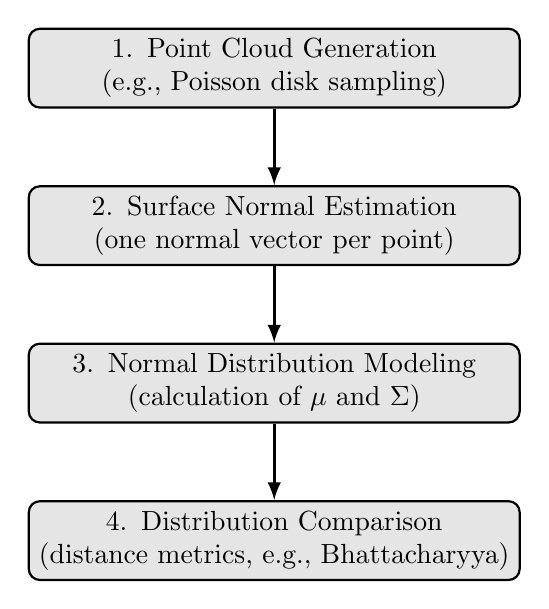
\begin{tikzpicture}[node distance=1cm, auto, thick]
        % Define a style for the nodes
        \tikzstyle{mybox} = [rectangle, draw, fill=gray!20, text width=6cm, text centered, rounded corners, minimum height=1cm]
        \tikzstyle{arrow} = [->, very thick, >=latex]

        % Nodes
        \node (start) [mybox] {1. Point Cloud Generation\\ (e.g., Poisson disk sampling)};
        \node (normals) [mybox, below of=start, yshift=-1cm] {2. Surface Normal Estimation\\(one normal vector per point)};
        \node (distribution) [mybox, below of=normals, yshift=-1cm] {3. Normal Distribution Modeling\\ (calculation of $\mu$ and $\Sigma$)};
        \node (comparison) [mybox, below of=distribution, yshift=-1cm] {4. Distribution Comparison\\ (distance metrics, e.g., Bhattacharyya)};

        % Edges
        \draw [arrow] (start) -- (normals);
        \draw [arrow] (normals) -- (distribution);
        \draw [arrow] (distribution) -- (comparison);
    \end{tikzpicture}
    \caption{Diagram of the workflow for comparing 3D objects through normal distributions.}
    \label{fig:method_diagram}
\end{figure}

\paragraph{Statistical Embedding}
A multivariate normal distribution is characterized by a mean vector $\boldsymbol{\mu}$ and a covariance matrix $\Sigma$. The mean vector represents the central tendency of the surface normals, while the covariance matrix captures the spread and correlations between the normal components. 

This process effectively converts a complex 3D object into a compact, low-dimensional statistical representation, which we refer to as a "statistical embedding". This embedding, comprised of the mean vector and covariance matrix, serves as the basis for our similarity comparisons.
\begin{figure}[H]
    \centering
    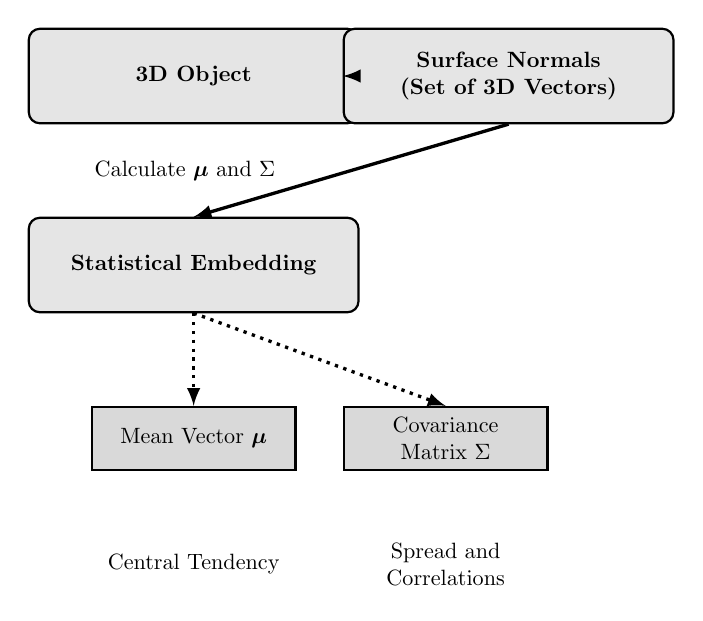
\begin{tikzpicture}[node distance=2cm, auto, thick, scale=0.8, every node/.style={transform shape}]
        % Define styles
        \tikzstyle{mybox} = [rectangle, draw, fill=gray!20, text width=5cm, text centered, rounded corners, minimum height=1.5cm, font=\bfseries]
        \tikzstyle{vector} = [rectangle, draw, fill=gray!30, text width=3cm, text centered, minimum height=1cm]
        \tikzstyle{matrix} = [rectangle, draw, fill=gray!30, text width=3cm, text centered, minimum height=1cm]
        \tikzstyle{arrow} = [->, very thick, >=latex]

        % Nodes
        \node (object) [mybox] {3D Object};
        
        \node (normals) [mybox, right of=object, xshift=3cm] {Surface Normals\\(Set of 3D Vectors)};

        \node (embedding) [mybox, below of=object, yshift=-1cm] {Statistical Embedding};
        
        \node (mu) [vector, below of=embedding, yshift=-0.75cm] {Mean Vector $\boldsymbol{\mu}$};
        \node (sigma) [matrix, right of=mu, xshift=2cm] {Covariance Matrix $\Sigma$};
        
        % Connections
        \draw [arrow] (object.east) -- (normals.west);
        
        \draw [arrow] (normals.south) -- node[left, midway, xshift=-1cm, text width=3cm, align=center] {Calculate $\boldsymbol{\mu}$ and $\Sigma$} (embedding.north);
        
        \draw [arrow, dotted] (embedding.south) -- (mu.north);
        \draw [arrow, dotted] (embedding.south) -- (sigma.north);

        % Explanations
        \node[below of=mu, yshift=0cm, text width=3cm, align=center] {Central Tendency};
        \node[below of=sigma, yshift=0cm, text width=3cm, align=center] {Spread and Correlations};

    \end{tikzpicture}
    \caption{Diagram of the statistical embedding process. A 3D object is first converted into a set of surface normals, which are then summarized by a mean vector $\boldsymbol{\mu}$ and a covariance matrix $\Sigma$ to form a compact statistical embedding.}
    \label{fig:statistical_embedding}
\end{figure}

The pseudocode for this estimation is as follows:
\begin{algorithm}[H]
\caption{Estimate Multivariate Normal Distribution}
\label{algorithm:estimate-mvn}
\begin{algorithmic}[1]
\Require
  \Statex $normals$: A list or array of surface normal vectors for a 3D object
  \Statex $n$: Number of normal vectors
  \Statex $dim$: Dimension of the normal vectors (e.g., 3 for 3D)
\Ensure
  \Statex $mean$: Mean vector
  \Statex $cov\_matrix$: Covariance matrix
\Function{estimateMultivariateNormalDistribution}{$normals, n, dim$}
  \State $mean \gets$ array of zeros with dimensions $(dim,)$
  \State $covariance\_matrix \gets$ 2D array of zeros with dimensions $(dim, dim)$
  \For{$i$ from $1$ to $n$}
    \State $mean \gets mean + normals[i]$
  \EndFor
  \State $mean \gets mean / n$
  \For{$i$ from $1$ to $n$}
    \State $diff \gets normals[i] - mean$
    \State $covariance\_matrix \gets covariance\_matrix + (diff \cdot diff^T)$
  \EndFor
  \State $covariance\_matrix \gets covariance\_matrix / (n - 1)$
  \State \Return $mean, covariance\_matrix$
\EndFunction
\end{algorithmic}
\caption{Code to describe a surface normal as a multivariate normal distribution}
\end{algorithm}



\subsection{Similarity Metrics}
To quantify the similarity between two 3D objects, we compare their respective multivariate normal distributions. We primarily use the **Bhattacharyya distance** \cite{Bhattacharyya} due to its effectiveness in measuring the overlap between two probability distributions. The Bhattacharyya distance $D_B(N_A, N_B)$ between two distributions $N_A$ and $N_B$ is computed as:
\[
D_B(N_A, N_B) = \frac{1}{8} (\boldsymbol{\mu}_B - \boldsymbol{\mu}_A)^T \Sigma^{-1} (\boldsymbol{\mu}_B - \boldsymbol{\mu}_A) + \frac{1}{2} \ln \left(\frac{\det(\Sigma)}{\sqrt{\det(\Sigma_A) \det(\Sigma_B)}}\right)
\]
where $\Sigma = (\Sigma_A + \Sigma_B) / 2$. A lower Bhattacharyya distance indicates greater similarity.

Additionally, we evaluate other common distance metrics for comparison:
\begin{itemize}
    \item \textbf{Mahalanobis Distance} \cite{Mahalanobis}: Measures the distance between a point and a distribution, or between two distributions, accounting for the data's variance.
    \item \textbf{Jensen-Shannon Divergence} \cite{JensenShannon}: A symmetric and smoothed version of the Kullback-Leibler divergence, used to measure the difference between two probability distributions.
\end{itemize}

\subsection{Deep Learning Comparison}
To contextualize the performance of our method, we compare it against a deep learning-based approach. We use a pretrained model, specifically PointGPT-S \cite{PointGPT}, a GPT-like model for point clouds. Instead of using the model for its original purpose of point recreation, we intercept its forward pass to extract a vector representation (embedding). These vector embeddings, typically of higher dimensionality (e.g., 384 dimensions), are then used to perform similarity queries via cosine similarity. This comparison allows us to evaluate the trade-offs between a feature-rich, data-driven representation and our computationally light, statistical approach.

\section{Experimental Results}

\subsection{Benchmark Setup}
The experiments were conducted using the ShapeNet dataset \cite{ShapeNet}. Our primary goal was to measure the effectiveness and computational efficiency of our statistical method against the deep learning model. The statistical embedding for our method was composed of 30 dimensions, based on statistical calculations of the surface normals for each dimension, including the covariance matrix, standard deviation, and percentiles.

\begin{table}[H]
    \centering
    \begin{tabular}{c|c}
        \toprule
        Artifact & version\\
        \midrule
        Python & 3.9.16\\
        Matplotlib & 3.8.0\\
        Open3d & 0.14.1\\
        IPython & 8.14.0\\
        Numpy & 1.25.2\\
        scipy & 1.11.3\\
        \bottomrule
    \end{tabular}
    \caption{Software requirements for reproducing the results}
    \label{tab:my_label}
\end{table}

\subsection{Performance Metrics}
We evaluated both methods using standard information retrieval metrics: **recall@k** and **mean average precision (mAP@k)**. The goal was to check the retrieval of shapes with the same taxonomy as the query shape.

\begin{figure}[H]
    \centering
    \includegraphics[width=1\linewidth]{pics/image.png}
    \caption{Recall and mAP metrics for both approaches}
\end{figure}

The results show that the AI method has a slightly better performance. This can be attributed to the fact that the AI model was trained on the ShapeNet training set, introducing a potential bias that contributes to its better performance on the test set.

\subsection{Computational Efficiency}
A key advantage of our statistical method is its computational efficiency. The 30-dimensional statistical embeddings are extremely fast to compute and require negligible storage. This allows for near real-time similarity searches, a task that would be significantly slower using the full forward pass of a complex deep learning model. Furthermore, our embeddings can be generated quickly on a CPU, eliminating the need for a dedicated GPU.

\subsection{Empirical Example}
Given the following three objects, our method provides a distance matrix for comparison:
\begin{figure}[!htb]
\minipage{0.32\textwidth}
  \includegraphics[width=\linewidth]{pics/chair_cp.jpg}
\endminipage\hfill
\minipage{0.32\textwidth}
  \includegraphics[width=\linewidth]{pics/spare_part_1_cp.jpg}
  \caption{Algorithm input surfaces}
\endminipage\hfill
\minipage{0.32\textwidth}%
  \includegraphics[width=\linewidth]{pics/spare_part_2_cp.jpg}
\endminipage
\end{figure}

\begin{table}[H]
    \centering
    \begin{tabular}{c|c|c|c}
        \toprule
                & chair & spare part 1 & spare part 2\\
        \midrule
         chair & - & (30.74, 41.69) & (30.49, 45.78)\\
        \midrule
         spare part 1 & (30.74, 41.69) & - & (19.14, 0.00)\\
        \midrule
         spare part 2 & (30.49, 45.78) & (19.14, 0.00) & -\\
        \bottomrule
    \end{tabular}
    \caption{Distances comparing normal surfaces, (not normalized, normalized)}
    \label{tab:my_label}
\end{table}

\section{Discussion and Future Work}
Our findings indicate that a statistical representation based on surface normal distributions provides a highly efficient and effective alternative to deep learning for 3D object recognition. While a pretrained AI model may offer slightly higher accuracy, our method excels in computational speed and resource requirements, making it an ideal choice for applications where these factors are critical, such as quality assessment or IP field analysis.

For future work, we suggest exploring the integration of generative AI models with our statistical representations. This hybrid approach could address challenges like surface deformations by generating plausible variations of an object consistent with its learned statistical properties. By combining the efficiency of our method with the robust deformation handling of generative models, we can further enhance the accuracy and reliability of 3D object comparison.

\section{Conclusion}
We have demonstrated a method for comparing 3D surfaces using estimated normal distributions, providing a robust and fast approach for object recognition. Our statistical embedding, coupled with distance metrics like Bhattacharyya, offers a powerful tool for analyzing surface similarity with minimal computational overhead. This work paves the way for advancements in 3D object analysis and recognition, particularly in scenarios where rapid and scalable comparisons are essential.

\bibliographystyle{plainnat}
 \bibliography{references}

\end{document}